%%%%%%%%%%%%%%%%%%%%%%%%%%%%%%%%%%%%%%%%%
% Structured General Purpose Assignment
% LaTeX Template
%
% This template has been downloaded from:
% http://www.latextemplates.com
%
% Original author:
% Ted Pavlic (http://www.tedpavlic.com)
%
% Note:
% The \lipsum[#] commands throughout this template generate dummy text
% to fill the template out. These commands should all be removed when
% writing assignment content.
%
%%%%%%%%%%%%%%%%%%%%%%%%%%%%%%%%%%%%%%%%%

%----------------------------------------------------------------------------------
%   PACKAGES AND OTHER DOCUMENT CONFIGURATIONS
%----------------------------------------------------------------------------------

\documentclass{article}

\usepackage{fancyhdr} % Required for custom headers
\usepackage{lastpage} % Required to determine the last page for the footer
\usepackage{graphicx} % Required to insert images
\usepackage{enumitem}
\usepackage{multicol}
\usepackage{environ}
\usepackage{caption}
\usepackage{hyperref}
\usepackage{calc}
\usepackage[utf8]{inputenc}
\usepackage[spanish]{babel}
\selectlanguage{spanish}
\addto\extrasspanish{%
    \def\figureautorefname{Figura}%
}

% Margins
\topmargin=-0.45in
\evensidemargin=0in
\oddsidemargin=0in
\textwidth=6.5in
\textheight=9.0in
\headsep=0.25in

\linespread{1.1} % Line spacing

% Set up the header and footer
\pagestyle{fancy}
\lhead{\small \hmwkClass: \hmwkTitle} % Top left header
\chead{} % Top center header
\rhead{\small \hmwkAuthorName} % Top right header
\lfoot{} % Bottom left footer
\cfoot{} % Bottom center footer
\rfoot{Página\ \thepage\ de\ \pageref{LastPage}} % Bottom right footer
\renewcommand\headrulewidth{0.4pt} % Size of the header rule
\renewcommand\footrulewidth{0.4pt} % Size of the footer rule

\setlength\parindent{0pt} % Removes all indentation from paragraphs

\newlength\widest
\makeatletter
\NewEnviron{ldescription}{%
    \vbox{%
        \global\setlength\widest{0pt}%
        \def\item[##1]{%
            \settowidth\@tempdima{\textbf{##1}}%
            \ifdim\@tempdima>\widest\global\setlength\widest{\@tempdima}\fi%
        }%
        \setbox0=\hbox{\BODY}%
    }
    \begin{description}[leftmargin=\dimexpr\widest+0.5em\relax,labelindent=16pt,labelwidth=\widest]
        \BODY
\end{description}%
}
\makeatother

%----------------------------------------------------------------------------------
%   NAME AND CLASS SECTION
%----------------------------------------------------------------------------------

\newcommand{\hmwkTitle}{Práctica\ 2} % Assignment title
\newcommand{\hmwkClass}{Sistemas Informáticos I} % Course/class
\newcommand{\hmwkClassTime}{10:30am} % Class/lecture time
\newcommand{\hmwkAuthorName}{\small Sergio Fuentes de Uña | Daniel Perdices Burrero} % Your name

%----------------------------------------------------------------------------------
%   TITLE PAGE
%----------------------------------------------------------------------------------

\title{
    \vspace{2in}
    \textmd{\textbf{\hmwkClass:\ \hmwkTitle}}\\
    \normalsize\vspace{0.1in}\small{\today}\\
    \vspace{3in}
}

\author{\textbf{\hmwkAuthorName}}
\date{} % Insert date here if you want it to appear below your name

%----------------------------------------------------------------------------------

\begin{document}

\maketitle

%----------------------------------------------------------------------------------
%   TABLE OF CONTENTS
%----------------------------------------------------------------------------------

%\setcounter{tocdepth}{1} % Uncomment this line if you don't want subsections listed in the ToC

\newpage
\tableofcontents
\newpage

\section{Archivos}
La entrega final de la práctica está compuesta por los siguientes archivos:
\begin{ldescription}
    \item[$\bullet$ \texttt{index.php}]
        Página principal del sitio web ({\small\autoref{fig:fig1}}).
    \item[$\bullet$ \texttt{matches.php}]
        Listado de partidos disponibles para apostar ({\small\autoref{fig:fig1}, \autoref{fig:fig2}, \autoref{fig:fig3}}).
    \item[$\bullet$ \texttt{register.php}]
        Formulario de registro de un nuevo usuario.
    \item[$\bullet$ \texttt{bet.php}]
        Formulario de realización de una apuesta.
    \item[$\bullet$ \texttt{checkout.php}]
        Administración del carrito de apuestas.
    \item[$\bullet$ \texttt{credit.php}]
        Administración de saldo del usuario.
    \item[$\bullet$ \texttt{history.php}]
        Historial de apuestas del usuario.
    \item[$\bullet$ \texttt{usercount.php}]
        Banner con número de usuarios conectados.
    \item[$\bullet$ \texttt{theme.css}]
        Hoja de estilo CSS del sitio web.
    \item[$\bullet$ \texttt{functions.js}]
        Librería de funciones JavaScript.
    \item[$\bullet$ \texttt{db.xml}]
        Conjunto de apuestas disponibles en XML.
    \item[$\bullet$ \texttt{users/}]
        Directorio de datos de los usuarios.
    \item[$\bullet$ \texttt{games/}]
        Directorio de recursos gráficos para las apuestas.
    \item[$\bullet$ \texttt{images/}]
        Directorio de recursos gráficos de propósito general.
    \item[$\bullet$ \texttt{Memoria-P2.pdf}]
        Memoria del trabajo realizado (este archivo).
\end{ldescription}
\newpage
\section{Instrucciones de uso}
\subsection{Encontrar una apuesta}
Al acceder a la página principal se muestra el conjunto de todas las apuestas, organizadas en dos secciones:
\begin{multicols}{2}
    \textbf{\textit{Upcoming Matches}}: Encuentros que aún no se han celebrado o que aún no han terminado y por los que se puede apostar, los más inminentes aparecen primero.
    \begin{minipage}{\linewidth}
        \centering
        \captionsetup{type=figure}
        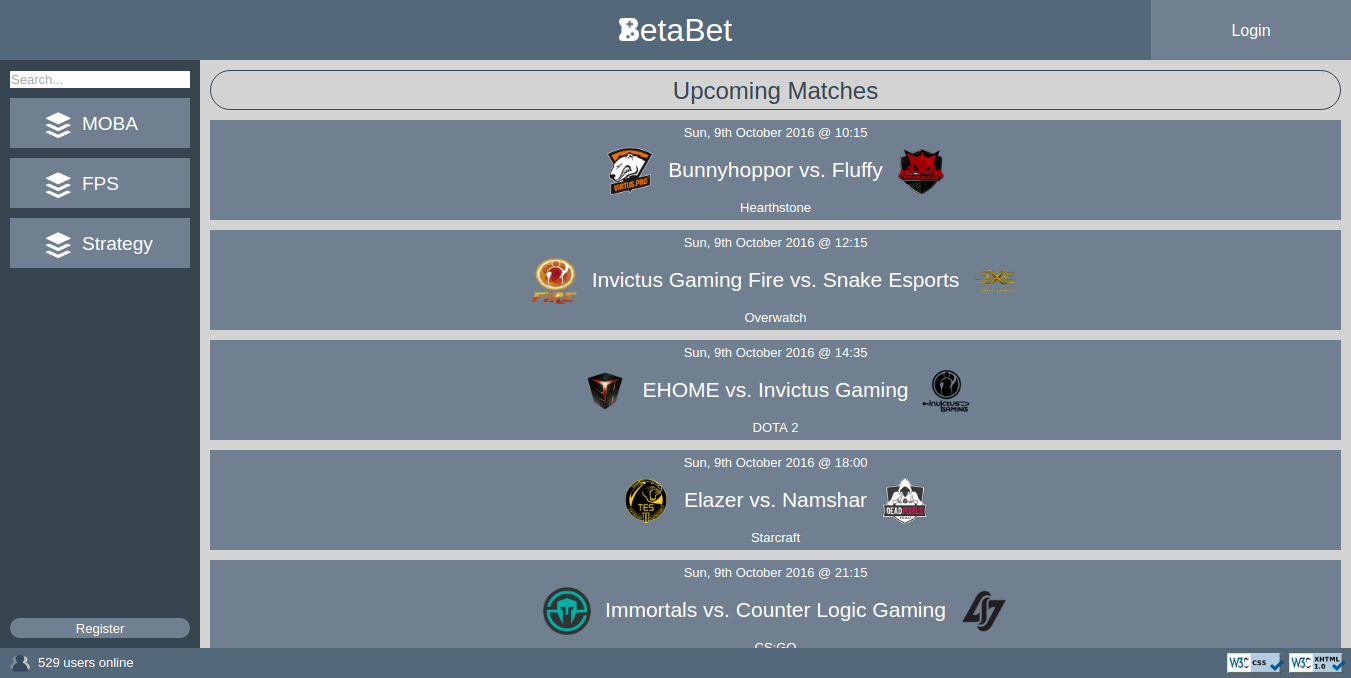
\includegraphics[width=\linewidth]{fig1}
        \caption{\textit{Upcoming Matches}}
        \label{fig:fig1}
    \end{minipage}
    \columnbreak\newline
    \textbf{\textit{Latest Matches}}: Encuentros finalizados por los que ya no es posible apostar y cuyos resultados se indican en la página, los más recientes aparecen primero.
    \begin{minipage}{\linewidth}
        \centering
        \captionsetup{type=figure}
        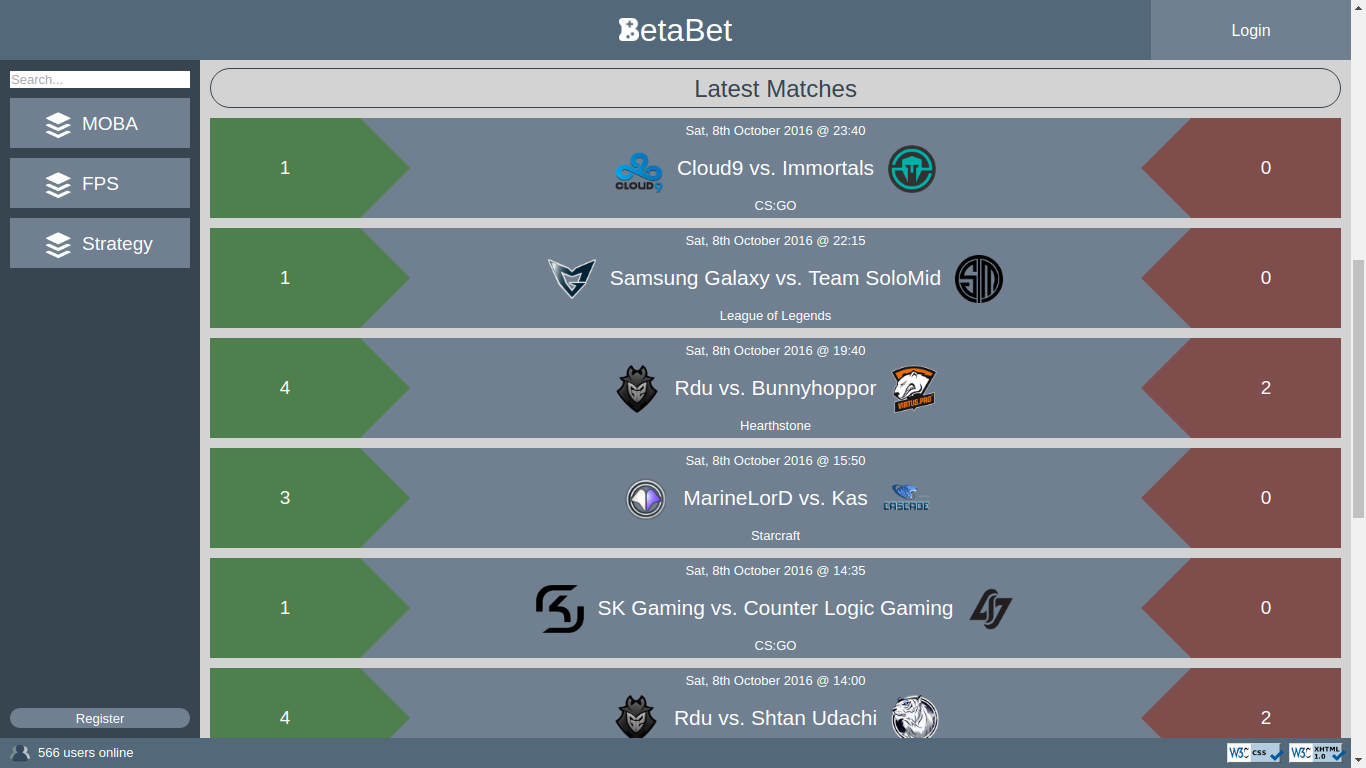
\includegraphics[width=\linewidth]{fig2}
        \caption{\textit{Latest Matches}}
        \label{fig:fig2}
    \end{minipage}
\end{multicols}
Existen dos mecanismos de filtrado de apuestas para localizar encuentros determinados de manera sencilla:
\begin{multicols}{2}
    \textbf{Categorías}: Desplegando los menús de la barra lateral y pulsando los botones correspondientes es posible filtrar las apuestas por categoría.
    \begin{minipage}{\linewidth}
        \centering
        \captionsetup{type=figure}
        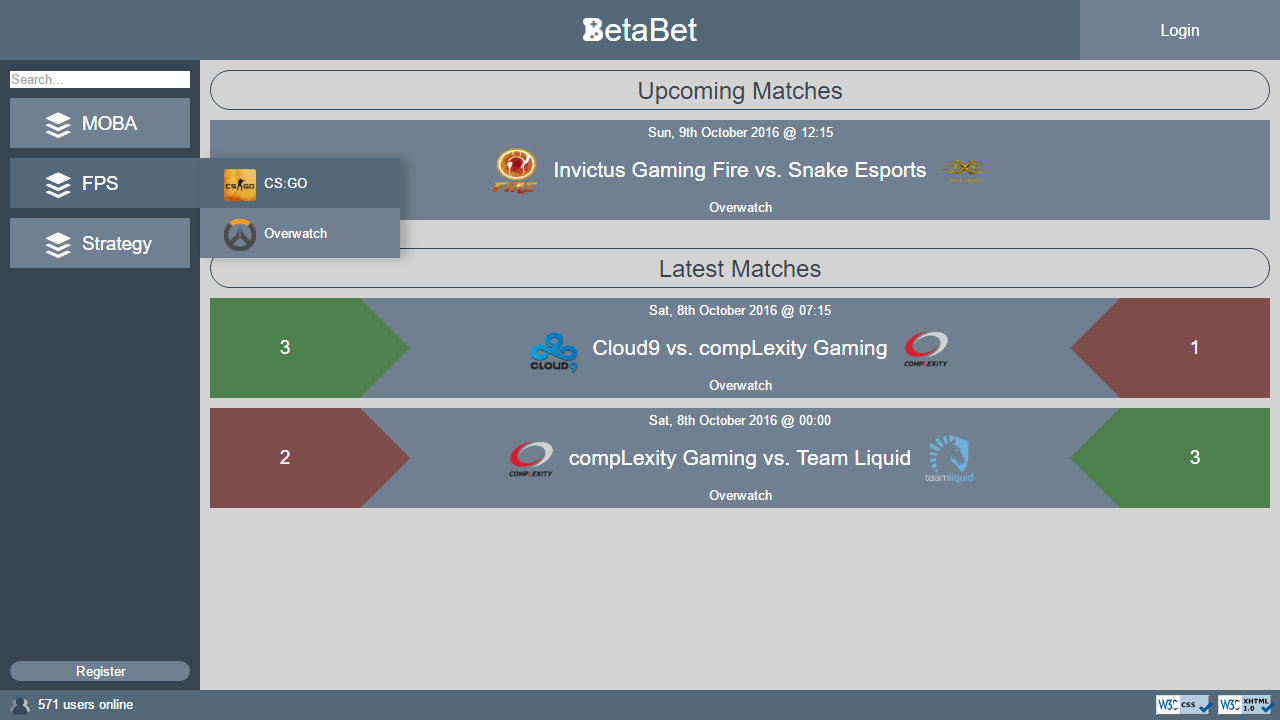
\includegraphics[width=\linewidth]{fig3}
        \caption{Filtrado por categorías}
        \label{fig:fig3}
    \end{minipage}
    \columnbreak\newline
    \textbf{Búsqueda}: Encuentros finalizados por los que ya no es posible apostar y cuyos resultados se indican en la página, los más recientes aparecen primero.
    \begin{minipage}{\linewidth}
        \centering
        \captionsetup{type=figure}
        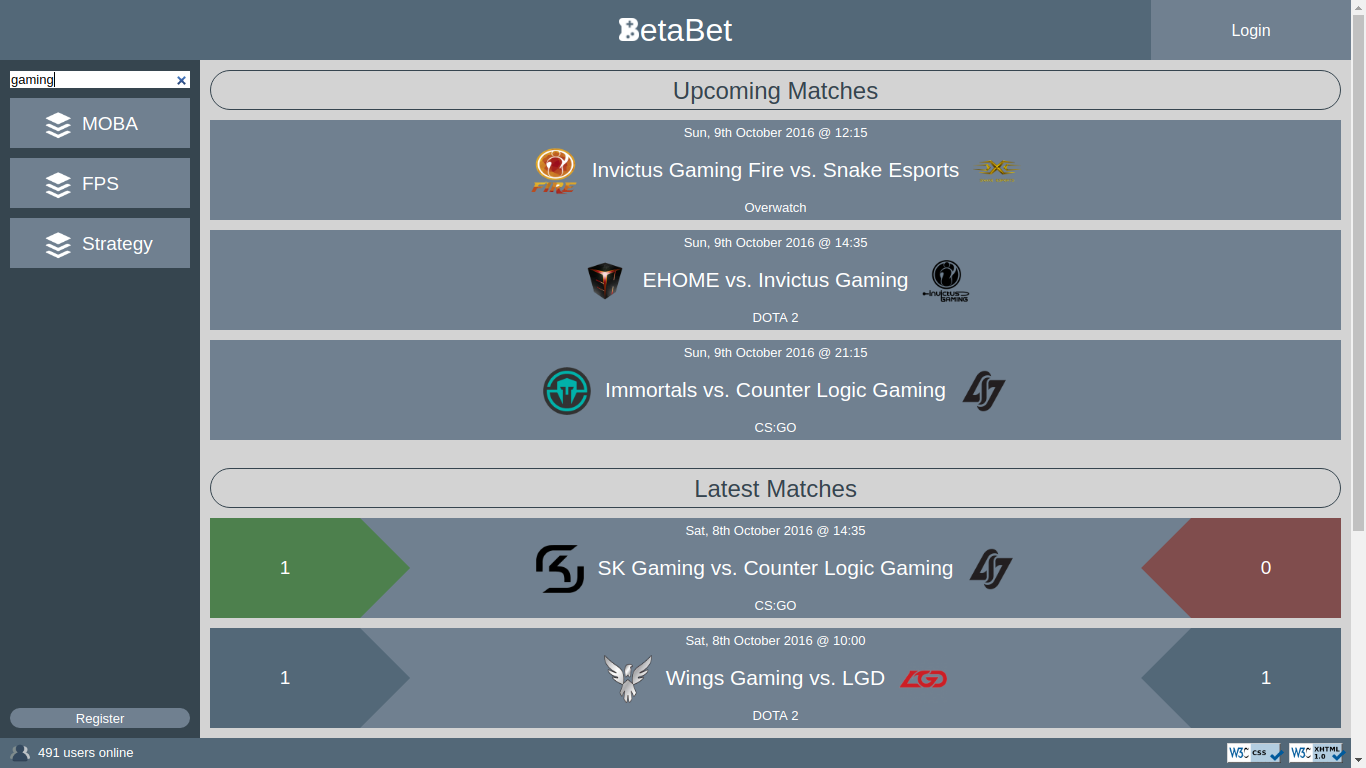
\includegraphics[width=\linewidth]{fig4}
        \caption{Filtrado por búsqueda}
        \label{fig:fig4}
    \end{minipage}
\end{multicols}
\newpage
\subsection{Realizar una apuesta}
\subsection{Confirmar el carrito}
\subsection{Registrar un nuevo usuario}
\subsection{Iniciar sesión con un usuario}
\subsection{Consultar saldo de la cuenta}
\subsection{Ingresar o retirar saldo}
\subsection{Consultar el historial de apuestas}
\section{Implementación}
\section{Referencias}

\end{document}
